\documentclass{article}
\title{CSCI 447 Project 3 Design Document}
\author{George Engel, Troy Oster, Dana Parker, Henry Soule}

\usepackage{hanging}
\usepackage{graphicx}

\begin{document}
\maketitle

\section{Introduction}
For this assignment, we are required to assess the performance of two neural networks on six different data sets.
The two neural networks implemented are (1) a multi-layer feedforward network with backpropagation learning and (2) a radial basis function neural network.
Our radial basis function neural network uses as its hidden layer the centroids from $k$-means clustering, the medoids from $k$-medoids clustering, and the reduced training set from either edited or condensed nearest neighbors (whichever of edited/condensed has less examples).

We hypothesize that the convergence rate for our feedforward neural network will be greater than our radial basis neural network because we will backpropagate upon potentially multiple hidden layers across multiple mini-batches, while the radial basis neural network backpropagates upon just one hidden layer of just one collection of neurons, the latter amounting to generally less operations to converge by than the former.
We also hypothesize that the feedforward neural network will be more accurate at both classification and regression than then radial basis function neural network because the radial basis neural network is limited to one hidden layer, unlike the feedforward neural network.

\section{Class Descriptions}

\begin{centering}
    \makebox[\textwidth]{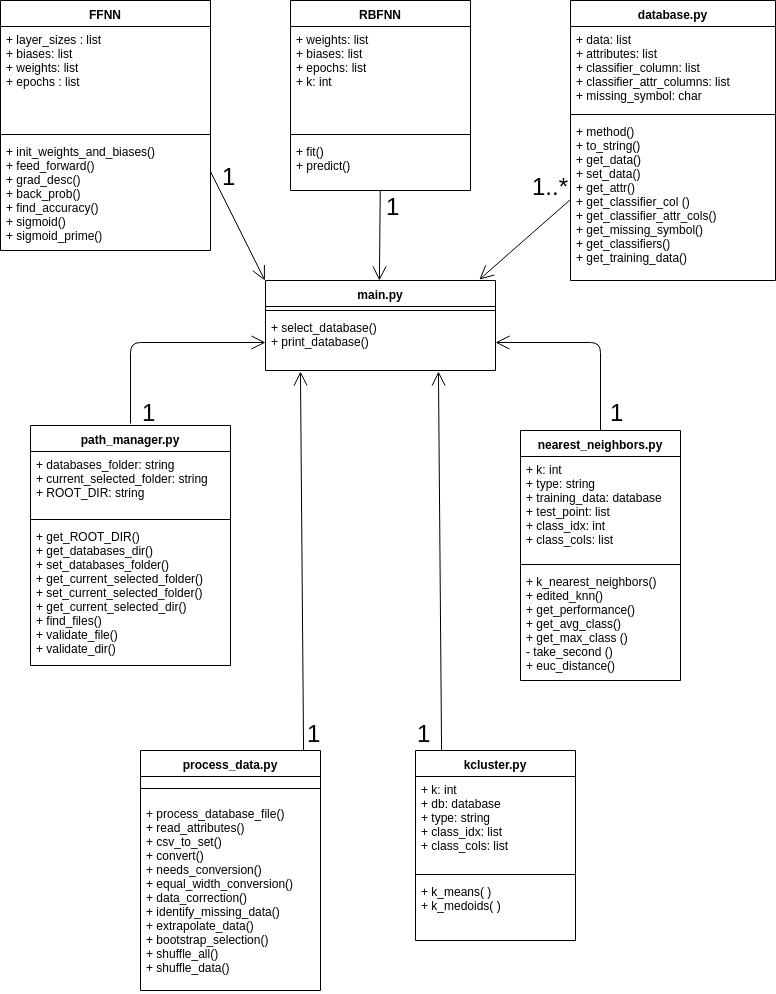
\includegraphics[width=4.75in]{uml.png}}
    \caption{\label{test} Figure 1: UML Diagram of All Diagrams}
\end{centering}

\newpage

\subsection*{path\_manager.py}
\texttt{path\_manager.py} handles pathing through the project's databases. This way it is easy to reconfigure or setup for a new database or file type at a moment's notice.

\subsection*{database.py}
\texttt{database.py} acts as an instantiable object for holding relevant information from a selected database (project data files).

\subsection*{process\_data.py}
\texttt{process\_data.py} targets a specified database, then loads in the relevant information from that database, then loads in the relevant information from that database's directory into a database object which can then be manipulated as we please. This class also contains functionality for identifying and correcting missing values from a database via bootstrapping. It also contains functionality for randomly shuffling the data of a given database by specific attribute and percentage to modify.

\subsection*{nearest\_neighbors.py}

Rather than having edited and condensed nearest neighbors algorithms in a class as we did previously, this time around we decided it best to implement them as static functions in a single file that we will call \texttt{nearest\_neighbors.py}. We do this so we invoke edited and condensed nearest neighbors functionality without having to reference a specific object. By removing the need to create a specific object to access edited and condensed nearest neighbor functionality, we also remove the inter-dependencies upon various class variables that gave us trouble previously.

The functionality of edited and condensed nearest neighbors will remain largely the same as the previous project. We implement edited and condensed nearest neighbors to use the smaller of the two reduced training data sets as one of three inputs for our radial basis function neural network.

\subsection*{kcluster.py}

The \texttt{kcluster.py} file contains the functionality for performing $k$-means clustering and $k$-medoids clustering, which each take in the training data as an input and each output a set of centroids or medoids, respectively, for us to use back in \texttt{main.py}. Essentially, these functions will be used to reduce our training data to help avoid horrendous run time while retaining some semblance of accuracy.

\subsection*{main.py}
\texttt{main.py} will perform the execution of our program.

\subsection*{ffnn.py}
\texttt{ffnn.py} will store our \texttt{FFNN} class, which handles all functionality for our multi-layer feedforward neural network. It will contain class variables for the number of neurons in each layer, a vector of biases, a vector of weights, and a list of total cost per each epoch executed. This class will also contain the network's functionality for the feedforward process, backpropagation, stochastic gradient descent, mini-batching, and calculating cost, and accuracy evaluation [2].

\subsection*{rbf.py}
\texttt{rbf.py} will store our \texttt{RBFN} class, which handles all functionality for our radial basis function network. It will store as attributes an integer value for $k$ as the number of neurons in our hidden layer, the number of epochs, and a reference to our chosen activation function. The \texttt{fit} function will perform our forward and backpropagation for each epoch.

\section{Design Decisions}

\subsection*{Missing Data Handling}
When a data set is identified to have missing data, we identify the sets of data with missing attributes, and move them from the database's stored data matrix into a separate list of the sets of data with missing attributes. Once the missing data has been identified, we substitute values for the missing attribute via bootstrapping random values from the set of data that does not contain any missing attributes as our means of imputation.

We opted to never remove data, even if under a certain threshold, as we assumed it would be more likely to impact our results than including data that would be discredited if incorrect by other present data. 
Additionally, we don't have a static value to symbolize a missing value, but rather one must be specified for a given data set in the database directory's \texttt{.attr} file. This approach allows missing values to be considered a category of their own if necessary.

\subsection*{Identifying Categorical versus Continuous Data}
In order to determine how we should process data and eventually decide which activation functions to use when building our neural net, we will define each database as either Categorical or Continuous in the database's relevant .attr file.

\subsection*{Nearest Neighbors Distance Function}
We decided on Euclidean distance as our means of determining nearest neighbors, as Manhattan distance didn't seem to make much sense seeing as it isn't direct. 

\subsection*{Determining Neural Net Layers and Size of Each Layer}

Rather than inputting the amount of layers and assigning each layer an amount of neurons in the command line, we decided to set it in a configuration file. That way we only need to run the application and will not be required to enter the same input over and over for testing.

\subsection*{State Saving and State Information Viewing}
To simplify the process of evaluation our output from epoch to epoch, and to help debug, we decided to add save states after each Epoch by storing the relevant neural net object as a \texttt{.json} file. 

Be it for evaluating the effect of using a different algorithm at that point, or we want to continue running from a save state where a slight bug in an algorithm caused the program to crash previously. We could just reload and start from that save state to test if the algorithm is fixed as opposed to having to re-run the entire thing. Thus saving a large amount of time in the long run when debugging/testing code.

Also, since the object is just stored as a \texttt{.json} file, it would be easy to write another python script purely for the sake of viewing/manipulating the save state's information. This would prove useful for unit testing, as it is much easier to make sure each function takes input and spits out the correct output than to try and run the entire thing and guess where problems are stemming from.

\subsection*{Determining Convergence}
Both our \texttt{FFNN} and \texttt{RBFN} implementations will store as a class attribute an arbitrarily chosen maximum number of epochs for which to run. We have elected to run our experiments this way, rather than until convergence so we can observe any potential unexpected behavior in either of our models. That is, if our model appears to converge after a certain number of epochs, but then happens to subsequently diverge again, we would want to observe this behavior. Observing this sort of behavior in either or our models may help illuminate any bugs in either model we may not have been aware of.

\section{Experimental Design}

\subsection*{Radial Basis Function Network}
Based on the requirements of the assignment, our activation function for each neuron in the hidden layer of our radial basis function network will be the Gaussian: $exp(\frac{||x-\mu_i||^2}{\sigma})$, where $x$ is our input, $\mu_i$ is current centroid, and $\sigma_i$ is the standard deviation for the $i$th cluster [1]. To compute a predicted output for either classification or regression we apply weights between each neuron's activation and each output neuron. We will initialize these weights randomly, and use backpropagation to tune these weights over each epoch until we reach some arbitrary number of total epochs (well before which we assume the network will have already converged).

\subsection*{Feedforward Neural Network}

Our activation functions for our feedforward neural network will be sigmoidal for when the network is performing classification and linear for when the network is performing regression. To compute a predicted output for either classification or regression we apply weights between every neuron in one layer and the next. We will also apply one bias to each layer's weighted sum of activations. These weights and biases will be initialized randomly, and we will use backpropagation to tune these weights over each epoch until we reach some arbitrary number of total epochs (well before which we assume the network will have already converged) [2].

The sigmoidal activation function can be expressed as $\sigma(x) = \frac{1}{1 + e^{-x}}$ where $x$ is some real number, in this case the weighted sum of the activations of the previous layer plus some bias. The linear activation function is simply the weighted sum of the activations in the previous layer plus some bias with no sigmoidal activation function applied [2].

\subsection*{Evaluation}

In order to properly evaluate our implementations, we will split up our evaluation methods for regression- and classification-based problems into separate functions. This splitting is necessary seeing as we care about different evaluation methods for classification and regression.

To evaluate the performance of our neural networks when they are performing regression, we need a way of comparing the predicted continuous value to the actual continuous value. That being said, we also need a method of measuring our prediction accuracy that is robust to outliers. So to meet these criteria, we chose to use to calculate the averaged observed difference (AOD) between the desired output and the predicted output from our neural network. This calculation can be written as $AOD = \frac{1}{n} \sum_{i=1}^n | y_i - \hat{y}_i|$

As for the evaluation of the performance of our neural networks when they are performing classification, we need a way of comparing our predicted classification against the actual classification. To meet this criteria, we decided to look at the percentage of correctly classified examples given to our network as test data. This allows us to accurately assess the performance of the neural network's classification abilities.

\section{Works Cited}
\begin{hangparas}{.25in}{1}
[1] Militký, J. “Fundamentals of Soft Models in Textiles.” Soft Computing in Textile Engineering, 2011, pp. 45–102., doi:10.1533/9780857090812.1.45.

[2] Svozil, Daniel, Vladimir Kvasnicka, and Jiri Pospichal. "Introduction to multi-layer feed-forward neural networks." Chemometrics and intelligent laboratory systems 39.1 (1997): 43-62.

\end{hangparas}

\end{document}

% Chunky monkey